\documentclass[11pt]{article}
\usepackage[margin=1in]{geometry}
\usepackage{amsmath,amssymb}
\usepackage{booktabs}
\usepackage{graphicx}
\usepackage{natbib}
\usepackage[hidelinks]{hyperref}
\usepackage{xcolor}
\usepackage{caption}
\captionsetup{font=small}
\bibliographystyle{plainnat}
\newcommand{\kappaOne}{1.60}
\newcommand{\rsqOne}{-0.19}
\newcommand{\nOne}{22}
\newcommand{\maeOne}{0.18}
\newcommand{\rhoOne}{0.48}
\newcommand{\plugN}{21}
\newcommand{\plugMAE}{0.049}
\newcommand{\plugRho}{0.95}
\newcommand{\plugAgree}{30}
\newcommand{\plugTot}{32}
\newcommand{\plugMAEfive}{0.038}
\newcommand{\plugMAEnn}{0.059}
\newcommand{\negNF}{22}
\newcommand{\nDense}{24}
\newcommand{\recMed}{62}
\newcommand{\recMin}{32}
\newcommand{\recMax}{730}
\newcommand{\naiveMin}{-2.68}
\newcommand{\naiveMax}{-0.11}
\newcommand{\ssMin}{15}
\newcommand{\ssMax}{72}
\newcommand{\ssBmMax}{8}
\newcommand{\rqPosThree}{20}
\newcommand{\qDiffMax}{0.10}
\newcommand{\crossMin}{0.11}
\newcommand{\crossMax}{0.86}
\newcommand{\totKB}{446,641}
\newcommand{\totAsks}{23,703}
\newcommand{\totRep}{10,558}
\newcommand{\rqTurned}{9}
\newcommand{\recMedStill}{52}
\newcommand{\nStill}{15}
\newcommand{\recMinStill}{32}
\newcommand{\recMaxStill}{76}


\title{When Accepted Answers Become Evidence:\\Feedback Loops in Self-Updating Retrieval}
\author{Pavan Kumar Guthikonda\\
\small Independent researcher (M.Tech alumnus, BITS Pilani)\\
\small \texttt{pavansky143@gmail.com}}
\date{October 2026}

\begin{document}
\maketitle

\begin{abstract}
Retrieval-augmented support systems often write answers that users accept back into their own knowledge base, so that the next similar question can be answered from the resolved case. We study what this loop does on real data. We use all twelve CQADupStack forums (\totKB{} posts, \totAsks{} questions), take the duplicate links marked by each forum's community as ground truth, and replay real repeat questions through three retrievers (bge-small-en-v1.5, all-MiniLM-L6-v2, BM25). Only user acceptance is simulated: correct answers are accepted with probability 0.9 and wrong answers with probability $p_w$. We find three things. (1) For both dense retrievers, write-back helps when users reject most wrong answers and hurts once they accept more than a forum- and retriever-specific crossover rate $p^*$, which ranges from below 0.10 to about 0.86. At $p_w=0.95$ write-back is significantly worse than never writing back in \negNF{} of \nDense{} dense configurations. BM25 is almost unaffected, because short question titles rarely outscore full posts under BM25. (2) A one-parameter law based only on base accuracy does not predict $p^*$ ($R^2=\rsqOne$). An exact decomposition of the accuracy change into per-entry effects of correct and wrong entries gives a plug-in estimate that, calibrated at a single acceptance rate, predicts $p^*$ with mean absolute error \plugMAE{} on the \plugN{} configurations with an interior crossover. (3) Reopening wrongly accepted answers recovers part of the loss, but not all of it; adding quarantine of repeatedly rejected entries changes little. Label-free monitors do not do much better than the observed acceptance rate at telling harmful runs from harmless ones; disagreement with an independent retriever is close to chance. Code and cached results will be released.
\end{abstract}

\section{Introduction}
A common design for retrieval-augmented generation (RAG) \citep{lewis2020rag} in customer support and IT service management is to treat resolved cases as new knowledge: when a user accepts an answer, the question and the answer it received are stored, and later questions can retrieve that entry. The idea is reasonable. Repeat questions are common, and a stored case written in the user's own words may match the next repeat better than the original documentation does.

The same mechanism is also a feedback loop. Whatever the system retrieved, if accepted, becomes evidence for future retrieval. Users accept wrong answers for many reasons: the answer looks plausible, they give up, or they solve the problem another way and close the ticket. Each accepted wrong answer adds an entry that resembles the next question more than the correct document does. Related loops are known to degrade generative models trained on their own outputs \citep{shumailov2024collapse,alemohammad2024mad} and to distort recommender systems \citep{chaney2018confounding}, but we are not aware of a measurement of this loop for retrieval on real repeat questions.

This paper extends a two-page pilot (two forums, one retriever, five orders) to all twelve CQADupStack forums, three retrievers, top-1 and top-5 metrics, ten random orders and 20-round streams. Its contributions are:
\begin{enumerate}
\item \textbf{A measurement of the sign change.} On real repeat questions, naive write-back turns from helpful to harmful at a crossover acceptance rate $p^*$ for wrong answers. We report $p^*$ with bootstrap intervals for 36 forum--retriever pairs and show that it varies widely across forums and retrievers, and that a lexical retriever is nearly immune in this setting (Section~\ref{sec:results}).
\item \textbf{A simple model of the crossover that can be checked.} We show that a one-parameter law based on base accuracy does not fit, and derive a plug-in estimate from an exact decomposition of the accuracy change into per-entry effects. Measured at one acceptance rate, it predicts the crossover across configurations (Section~\ref{sec:model}).
\item \textbf{An honest account of safeguards and monitoring.} Reopening wrongly accepted answers recovers a median of \recMedStill\% of the loss where a loss remains. None of five label-free monitors, including disagreement with an independent retriever and drift on a fixed probe bank, separates harmful from harmless runs much better than the acceptance rate itself (Section~\ref{sec:monitor}).
\end{enumerate}

\section{Related work}
\paragraph{Self-consuming models.} \citet{shumailov2024collapse} show that generative models trained recursively on generated data lose the tails of the original distribution, and \citet{alemohammad2024mad} show that without enough fresh real data each generation of a self-consuming loop loses quality or diversity. Our setting differs in two ways: nothing is retrained, and the loop runs through human acceptance, so a correct entry can genuinely improve the system. The question is therefore not whether degradation occurs but where the balance tips.

\paragraph{Feedback loops in deployed ML.} \citet{sculley2015debt} list direct and hidden feedback loops as a source of technical debt. \citet{perdomo2020performative} formalise prediction that influences the outcome it predicts. \citet{chaney2018confounding} show in simulation that recommender feedback loops increase homogeneity without increasing utility, and \citet{ensign2018runaway} show runaway loops in predictive policing. Learning to rank from implicit feedback must correct for the bias the ranker itself introduces \citep{joachims2017unbiased}. Our loop is a direct one, where the system's output becomes part of its own index.

\paragraph{Knowledge-base poisoning.} PoisonedRAG \citep{zou2025poisonedrag} shows that a few crafted documents injected into a RAG knowledge base can steer answers. Write-back is an unintentional version of the same channel: the injected entries are written by the system and approved by ordinary users, not crafted by an adversary.

\paragraph{Data and retrievers.} CQADupStack \citep{hoogeveen2015cqadupstack} contains threads from twelve StackExchange forums with duplicate links marked by the community; we use the BEIR distribution \citep{thakur2021beir}. We use bge-small-en-v1.5 \citep{xiao2024cpack}, all-MiniLM-L6-v2 \citep{reimers2019sbert,wang2020minilm} and BM25 \citep{robertson2009bm25}.

\paragraph{Monitoring without labels.} Detecting shift without labels is studied by \citet{rabanser2019failing}; \citet{jiang2022disagreement} show that disagreement between independently trained models can track test error. We test the analogous idea of disagreement between the deployed retriever and an independent one.

\section{Setup}
\label{sec:setup}
\paragraph{Problem families.} For each CQADupStack test question, the community has marked one or more posts as duplicates. A question and its marked duplicates form a \emph{problem family}. The post with the lowest identifier (the oldest) stays in the knowledge base (KB) as the canonical thread; the test question and the titles of the other marked duplicates become \emph{asks} of the same problem. All other posts stay in the KB as distractors. An answer is correct only when the retrieved thread is the canonical thread of the ask's own family. Every ask is a real question written by a real user, and every wrong answer is a real retrieval error. Table~\ref{tab:data} gives the sizes.

\begin{table}[t]\centering\small
\begin{tabular}{lrrrr}\toprule Forum & KB posts & Asks & Families & Repeat asks\\\midrule
android & 22,001 & 1,696 & 699 & 997\\
english & 38,026 & 3,765 & 1,570 & 2,195\\
gaming & 44,633 & 2,263 & 1,595 & 668\\
gis & 37,408 & 1,114 & 885 & 229\\
mathematica & 16,151 & 1,358 & 804 & 554\\
physics & 37,422 & 1,933 & 1,039 & 894\\
programmers & 31,377 & 1,675 & 876 & 799\\
stats & 42,008 & 913 & 652 & 261\\
tex & 65,936 & 5,154 & 2,906 & 2,248\\
unix & 46,761 & 1,693 & 1,072 & 621\\
webmasters & 16,516 & 1,395 & 506 & 889\\
wordpress & 48,402 & 744 & 541 & 203\\
\midrule total & 446,641 & 23,703 & 13,145 & 10,558\\\bottomrule\end{tabular}
\caption{The twelve CQADupStack forums as used here. ``Repeat asks'' are asks of a family beyond its first ask.}
\label{tab:data}
\end{table}

\paragraph{Retrievers.} KB posts are embedded as title plus the first part of the body (1{,}200 characters). bge-small-en-v1.5 (512 tokens) and all-MiniLM-L6-v2 (256 tokens) are run with sentence-transformers, and retrieval is cosine similarity. BM25 uses $k_1=1.2$, $b=0.75$, English stop words removed. A written-back entry contains the ask text and points to the thread that was shown. For BM25, written-back entries are scored with the IDF and average length of the original KB; we do not update these statistics as entries are added, which is a small approximation.

\paragraph{The loop.} Asks arrive in a random order split into $R$ rounds ($R=10$; also $R=20$ on four forums). For each ask, the system shows the top-1 thread. A simulated user accepts a correct answer with probability $p_c=0.9$ and a wrong one with probability $p_w\in\{0.1,0.2,\dots,0.9,0.95\}$. Accepted answers are written back, and new entries become retrievable at the start of the next round (batch re-indexing). Four conditions are compared: \emph{no write-back}; \emph{naive} write-back; \emph{+demotion}, where half of the accepted wrong answers are reopened in the next round and their entries removed; and \emph{+demotion+quarantine}, where in addition any entry (original or written back) rejected twice is withdrawn. Safeguards are run at $p_w\in\{0.3,0.6,0.8,0.95\}$. The acceptance decision is the only simulated part.

\paragraph{Metrics and statistics.} We report top-1 accuracy over the whole stream and hit@5 (whether any of the top five entries points to the correct thread; the loop itself is driven by top-1). Each configuration is run with ten random orders. We report the paired difference from no write-back on the same order, in percentage points, with a 95\% $t$-interval over the ten orders. The crossover $p^*$ is the first $p_w$ at which the mean paired difference becomes negative, by linear interpolation on the grid; its 95\% interval comes from 1{,}000 bootstrap resamples of the orders. A crossover below the grid is reported as $<$0.10, and one above it as $>$0.95.

\section{Results}
\label{sec:results}

\begin{figure}[t]\centering
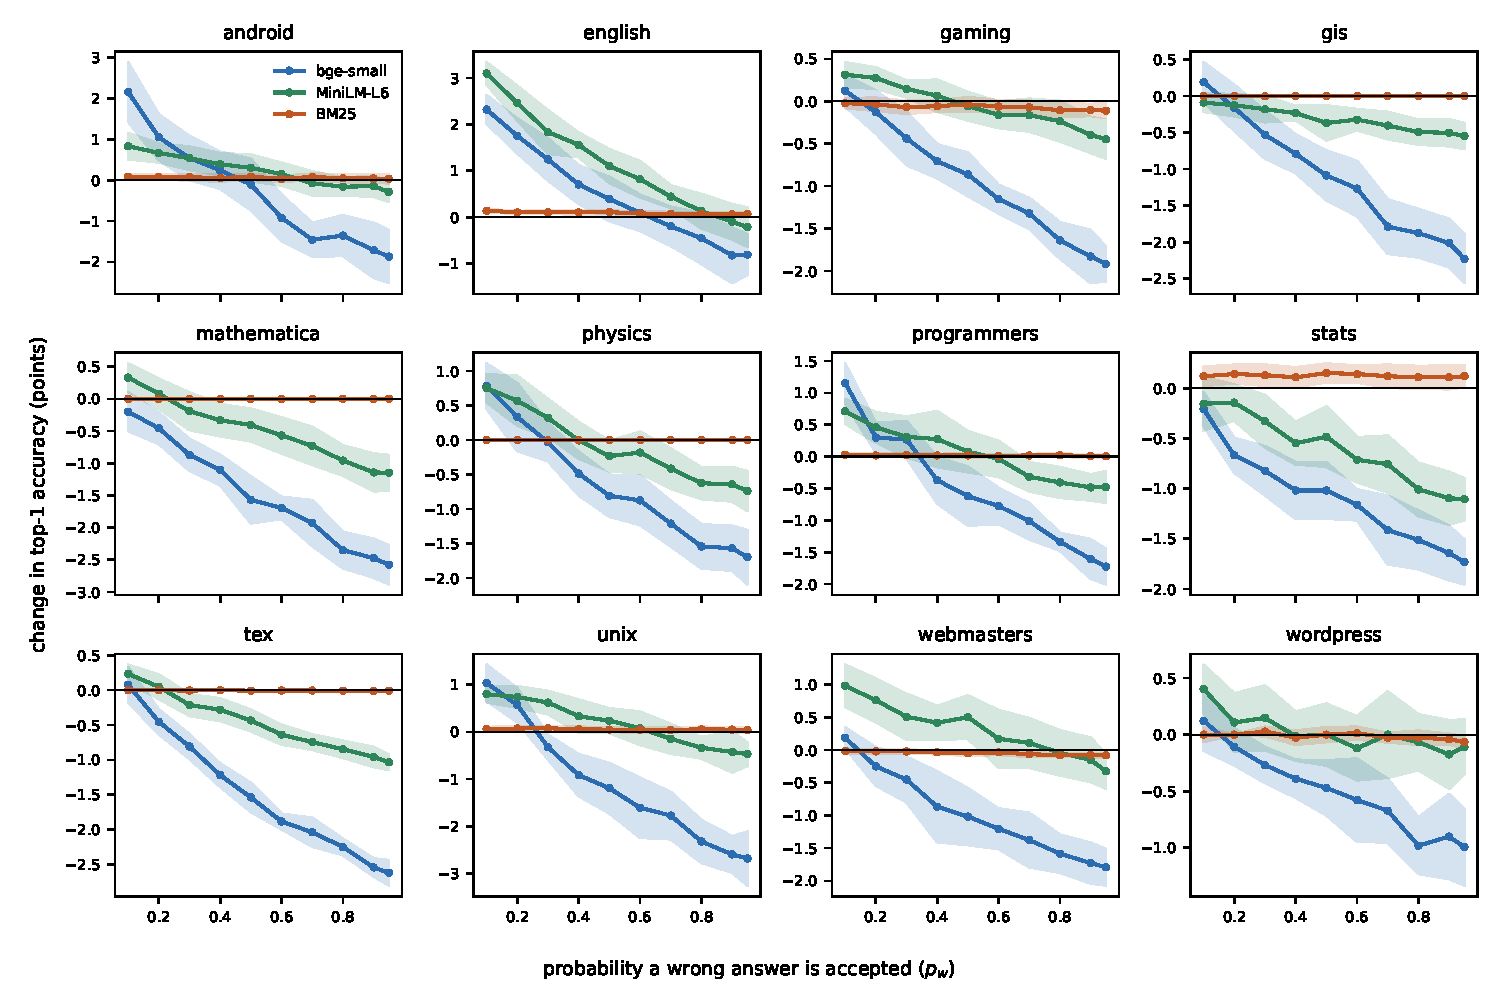
\includegraphics[width=\linewidth]{../figs/delta_r10_all.pdf}
\caption{Change in top-1 accuracy over the stream from naive write-back, relative to no write-back on the same order, as the acceptance rate of wrong answers grows. Bands are 95\% intervals over ten orders. Ten rounds.}
\label{fig:delta}
\end{figure}

\paragraph{The loop changes sign.} Figure~\ref{fig:delta} shows the paired change in top-1 accuracy for every forum and retriever. For both dense retrievers, the curve falls almost linearly with $p_w$ (median $R^2$ of a linear fit above 0.95). When users reject most wrong answers, write-back helps on most forums, by up to 3.1 points. When they accept nearly all of them, it hurts: at $p_w=0.95$ the change for dense retrievers ranges from \naiveMin{} to \naiveMax{} points, and the 95\% interval lies entirely below zero in \negNF{} of \nDense{} dense configurations. With base top-1 accuracies between 9\% and 35\% (Table~\ref{tab:cross}), a loss of 2.7 points is roughly a tenth of all correct answers. The pilot's numbers for Unix and Android are reproduced in direction and size (the pilot reported $-2.1$ and $-1.8$ points at $p_w=0.95$ with five orders; here $-2.68\pm0.57$ and $-1.87\pm0.65$ with ten orders, a re-computed embedding, and batch semantics that match the pilot).

\begin{table}[t]\centering\scriptsize
\begin{tabular}{llrrlll}\toprule Forum & Retriever & Top-1 & Hit@5 & Observed $p^*$ (top-1) & Observed $p^*$ (hit@5) & Plug-in $\hat p^*$\\\midrule
android & bge & 16.7 & 32.8 & 0.47 [0.37, 0.54] & 0.55 [0.39, 0.63] & 0.39\\
 & MiniLM & 22.3 & 38.9 & 0.67 [0.56, 0.78] & 0.67 [0.48, 0.89] & 0.69\\
 & BM25 & 13.7 & 23.0 & $>$0.95 & $>$0.95 & $>$0.95\\
\addlinespace[1pt]
english & bge & 19.1 & 34.2 & 0.63 [0.50, 0.75] & 0.39 [0.33, 0.44] & 0.61\\
 & MiniLM & 23.0 & 40.6 & 0.86 [0.77, 0.95] & 0.53 [0.46, 0.60] & 0.85\\
 & BM25 & 11.2 & 17.9 & $>$0.95 & 0.59 [0.37, 0.95] & $>$0.95\\
\addlinespace[1pt]
gaming & bge & 31.7 & 54.3 & 0.15 [0.10, 0.22] & $<$0.10 & 0.14\\
 & MiniLM & 34.7 & 57.0 & 0.45 [0.35, 0.56] & $<$0.10 & 0.49\\
 & BM25 & 27.0 & 41.1 & $<$0.10 & $<$0.10 & $<$0.10\\
\addlinespace[1pt]
gis & bge & 21.4 & 39.0 & 0.15 [0.10, 0.22] & 0.19 [0.16, 0.34] & 0.14\\
 & MiniLM & 25.2 & 44.4 & $<$0.10 & 0.31 [0.22, 0.41] & $<$0.10\\
 & BM25 & 16.8 & 29.9 & $>$0.95 & 0.10 [0.10, 0.40] & --\\
\addlinespace[1pt]
mathematica & bge & 12.1 & 26.1 & $<$0.10 & 0.12 [0.10, 0.19] & $<$0.10\\
 & MiniLM & 13.0 & 28.0 & 0.23 [0.17, 0.31] & 0.20 [0.15, 0.31] & 0.24\\
 & BM25 & 9.4 & 18.7 & $>$0.95 & $<$0.10 & --\\
\addlinespace[1pt]
physics & bge & 20.2 & 36.1 & 0.29 [0.19, 0.34] & 0.25 [0.18, 0.29] & 0.29\\
 & MiniLM & 21.5 & 40.4 & 0.40 [0.33, 0.47] & 0.28 [0.16, 0.37] & 0.45\\
 & BM25 & 13.5 & 24.3 & $>$0.95 & 0.20 [0.10, 0.40] & --\\
\addlinespace[1pt]
programmers & bge & 16.4 & 33.3 & 0.34 [0.30, 0.39] & 0.20 [0.17, 0.30] & 0.36\\
 & MiniLM & 17.4 & 34.3 & 0.57 [0.33, 0.66] & 0.56 [0.36, 0.73] & 0.47\\
 & BM25 & 11.6 & 20.1 & $>$0.95 & $<$0.10 & $>$0.95\\
\addlinespace[1pt]
stats & bge & 18.1 & 31.5 & $<$0.10 & 0.16 [0.11, 0.19] & $<$0.10\\
 & MiniLM & 20.2 & 35.7 & $<$0.10 & 0.35 [0.31, 0.41] & 0.11\\
 & BM25 & 15.8 & 24.9 & $>$0.95 & $>$0.95 & --\\
\addlinespace[1pt]
tex & bge & 11.5 & 22.7 & 0.11 [0.10, 0.14] & 0.14 [0.11, 0.16] & 0.13\\
 & MiniLM & 14.4 & 28.4 & 0.22 [0.16, 0.27] & 0.26 [0.21, 0.32] & 0.17\\
 & BM25 & 10.6 & 18.7 & 0.10 [0.10, 0.40] & $<$0.10 & $<$0.10\\
\addlinespace[1pt]
unix & bge & 20.8 & 36.3 & 0.26 [0.24, 0.29] & 0.28 [0.26, 0.31] & 0.24\\
 & MiniLM & 23.1 & 44.1 & 0.63 [0.50, 0.74] & 0.55 [0.45, 0.65] & 0.73\\
 & BM25 & 14.1 & 22.3 & $>$0.95 & $>$0.95 & $>$0.95\\
\addlinespace[1pt]
webmasters & bge & 10.8 & 21.1 & 0.14 [0.11, 0.19] & 0.16 [0.13, 0.19] & 0.16\\
 & MiniLM & 12.3 & 24.9 & 0.77 [0.56, 0.93] & 0.59 [0.50, 0.78] & 0.69\\
 & BM25 & 9.3 & 16.1 & $<$0.10 & 0.85 [0.57, 0.95] & $<$0.10\\
\addlinespace[1pt]
wordpress & bge & 14.0 & 27.8 & 0.15 [0.10, 0.20] & $<$0.10 & 0.13\\
 & MiniLM & 16.9 & 31.5 & 0.39 [0.17, 0.95] & $>$0.95 & 0.48\\
 & BM25 & 14.8 & 24.1 & 0.35 [0.10, 0.87] & 0.10 [0.10, 0.50] & 0.61\\
\bottomrule\end{tabular}
\caption{No-write-back accuracy (\%) and the crossover acceptance rate $p^*$ for naive write-back, with 95\% bootstrap intervals over ten orders. The last column is the plug-in prediction of Section~\ref{sec:model}, calibrated from the runs at $p_w=0.3$ only. ``--'': no entry ever changed an answer.}
\label{tab:cross}
\end{table}

\paragraph{The crossover is not a constant.} Table~\ref{tab:cross} lists $p^*$. Among dense configurations with an interior crossover it ranges from \crossMin{} to \crossMax{}. On some forums (stats, mathematica with bge, gis with MiniLM) write-back is harmful at every tested acceptance rate. The weaker MiniLM model often has a \emph{higher} crossover than bge on the same forum, so a better base retriever does not by itself make write-back safer. Crossovers for hit@5 are broadly similar but noisier. The intervals are wide in places (for example MiniLM on wordpress), because the curve is nearly flat there.

\paragraph{BM25 is nearly immune here.} With BM25, write-back changes accuracy by less than 0.2 points in every forum and condition, and written-back entries supply at most \ssBmMax\% of top-1 answers in the second half of the stream, against \ssMin--\ssMax\% for dense retrievers at $p_w=0.95$. The reason is visible before any simulation. For each ask we compare its score against the best original post with its score against the best other ask from the same family, as if that ask had been written back. Under bge, the other ask scores higher for 36--72\% of asks (depending on forum); under MiniLM for 20--49\%; under BM25 for only 2--12\%. Short titles share few terms with a new title and lose to long posts that match more terms. Dense encoders place two short titles close together whether or not they describe the same problem: under bge an ask from a \emph{different} family outscores the best original post for 33--74\% of asks. This is the mechanism of the takeover, and it also explains why most of the harm comes from wrong entries capturing questions they do not belong to. We do not claim BM25 is safe in general; with longer written-back entries (for example, the full generated answer) the picture may differ.

\begin{figure}[t]\centering
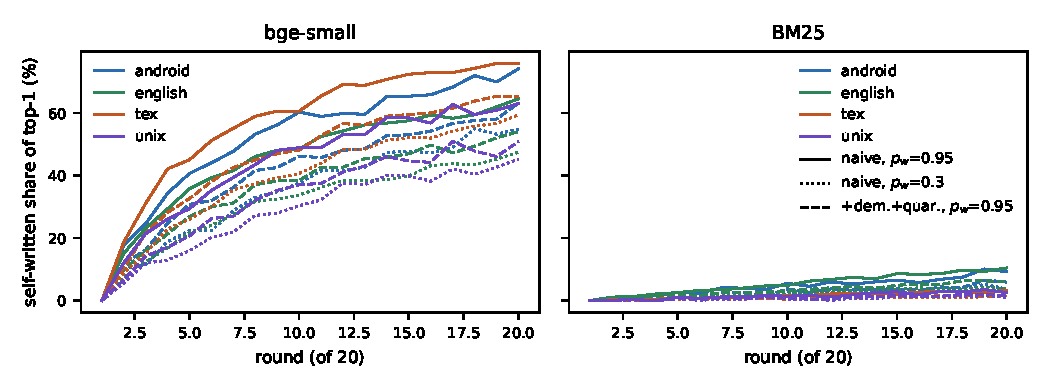
\includegraphics[width=0.85\linewidth]{../figs/selfshare_r20.pdf}
\caption{Share of top-1 answers that come from written-back entries over 20 rounds, averaged over ten orders. Left: bge-small. Right: BM25.}
\label{fig:selfshare}
\end{figure}

\paragraph{Self-written entries take over retrieval.} Figure~\ref{fig:selfshare} shows the takeover over 20 rounds. With bge and naive write-back at $p_w=0.95$, written-back entries supply more than half of all top-1 answers by round 9 to 13 (of 20) on all four forums, and 61--76\% by the end. Safeguards slow the takeover but do not stop it.

\paragraph{Longer streams.} Doubling the number of rounds to 20 on four forums leaves crossovers and losses within the intervals of the 10-round runs (Table~\ref{tab:r20}). The stream length in asks is the same; only the re-indexing interval is shorter. A longer stream of new asks would need more data than CQADupStack provides.

\begin{table}[t]\centering\scriptsize
\begin{tabular}{llllll}\toprule Forum & Retriever & $p^*$ (10 rounds) & $p^*$ (20 rounds) & Naive, $p_w{=}0.95$ (10) & (20)\\\midrule
android & bge & 0.47 [0.37, 0.54] & 0.45 [0.36, 0.53] & -1.87 $\pm$ 0.65 & -2.04 $\pm$ 0.69\\
 & MiniLM & 0.67 [0.56, 0.78] & 0.66 [0.55, 0.91] & -0.29 $\pm$ 0.24 & -0.29 $\pm$ 0.25\\
english & bge & 0.63 [0.50, 0.75] & 0.61 [0.50, 0.70] & -0.81 $\pm$ 0.44 & -0.84 $\pm$ 0.42\\
 & MiniLM & 0.86 [0.77, 0.95] & 0.82 [0.77, 0.95] & -0.21 $\pm$ 0.42 & -0.22 $\pm$ 0.48\\
tex & bge & 0.11 [0.10, 0.14] & 0.12 [0.10, 0.15] & -2.62 $\pm$ 0.18 & -2.73 $\pm$ 0.22\\
 & MiniLM & 0.22 [0.16, 0.27] & 0.22 [0.17, 0.27] & -1.03 $\pm$ 0.11 & -1.08 $\pm$ 0.10\\
unix & bge & 0.26 [0.24, 0.29] & 0.26 [0.22, 0.28] & -2.68 $\pm$ 0.57 & -2.95 $\pm$ 0.57\\
 & MiniLM & 0.63 [0.50, 0.74] & 0.63 [0.51, 0.77] & -0.47 $\pm$ 0.24 & -0.47 $\pm$ 0.32\\
\bottomrule\end{tabular}
\caption{Crossover and loss at $p_w=0.95$ with 10 and 20 rounds on four forums.}
\label{tab:r20}
\end{table}

\paragraph{Safeguards recover part of the loss.} Table~\ref{tab:safe} (Appendix~\ref{app:safe}) reports the paired change at $p_w=0.3$ and $0.95$ for the dense retrievers. At $p_w=0.3$, write-back with demotion and quarantine is positive in \rqPosThree{} of \nDense{} dense configurations. At $p_w=0.95$ it turns the loss into a non-negative change in \rqTurned{} of \nDense{} configurations. In the other \nStill{} it recovers a median of \recMedStill\% of the loss (range \recMinStill--\recMaxStill\%), so the loss is reduced but not removed. Quarantine adds very little on top of demotion: the two differ by at most \qDiffMax{} points at $p_w=0.95$. With a 90\% acceptance rate for correct answers, few entries are rejected twice before they have done their damage.


\section{A model of the crossover}
\label{sec:model}
\paragraph{An exact decomposition.} Under naive write-back no original post is ever withdrawn, so an answer can differ from the no-write-back answer only when the top-1 result is a written-back entry. Attributing each such change to the entry that caused it gives an exact identity
\begin{equation}
N\,\Delta = C\,\bar e_c + W\,\bar e_w,
\label{eq:decomp}
\end{equation}
where $N$ is the number of asks, $\Delta$ the change in accuracy, $C$ and $W$ the numbers of correct and wrong entries that were written and became retrievable, and $\bar e_c$ and $\bar e_w$ the average net number of answers each kind of entry turned from wrong to right (minus right to wrong). We count these quantities directly in the simulation.

\paragraph{First-order approximation.} If the system's accuracy on the asks that generate entries stays near its no-write-back accuracy $A$, then $C\approx p_c A N'$ and $W\approx p_w(1-A)N'$, with $N'$ the number of asks whose entries become retrievable. If the per-entry effects do not depend on $p_w$, setting $\Delta=0$ gives
\begin{equation}
p^* \approx \frac{p_c\,A}{1-A}\cdot\frac{\bar e_c}{-\bar e_w}.
\label{eq:pstar}
\end{equation}
Both assumptions are approximations: entries compete with each other, so per-entry effects shrink as more entries are written, and write-back itself changes the accuracy of later asks.

\paragraph{A one-parameter law does not fit.} If the ratio $\kappa=\bar e_c/(-\bar e_w)$ were the same everywhere, $p^*$ would be a function of base accuracy alone. Fitting a single $\kappa$ by least squares to the \nOne{} interior crossovers gives $\kappa=\kappaOne$ but $R^2=\rsqOne$ (Spearman $\rho=\rhoOne$; Figure~\ref{fig:cross}a). Base accuracy alone does not predict when write-back becomes harmful. Gaming has the highest base accuracy and one of the lowest crossovers for bge.

\paragraph{A plug-in estimate does.} The ratio $\kappa$ is specific to the forum and retriever: in our runs $\bar e_c$ ranges from about zero to $0.15$ answers gained per correct entry, while $\bar e_w$ lies between $-0.01$ and $-0.08$ (dense retrievers, $p_w=0.3$). Measuring $\bar e_c$ and $\bar e_w$ from the runs at a single acceptance rate ($p_w=0.3$) and inserting them into Eq.~\eqref{eq:pstar} predicts the crossover found from the full sweep with mean absolute error \plugMAE{} and Spearman $\rho=\plugRho$ over the \plugN{} configurations where both are interior. Prediction and observation agree, within the bootstrap interval ($\pm0.05$) or in the direction of censoring, for \plugAgree{} of \plugTot{} configurations where the estimate is defined (Figure~\ref{fig:cross}b, Table~\ref{tab:cross}). Calibrating at $p_w=0.5$ or $0.95$ instead gives mean absolute errors of \plugMAEfive{} and \plugMAEnn{}. This is an empirical check of a first-order model, not a proof. It does have a practical reading. The per-entry effects can be estimated in deployment from a small audited sample of written-back entries, and the deployment's own acceptance rate for wrong answers can then be compared against the predicted $p^*$.

\begin{figure}[t]\centering
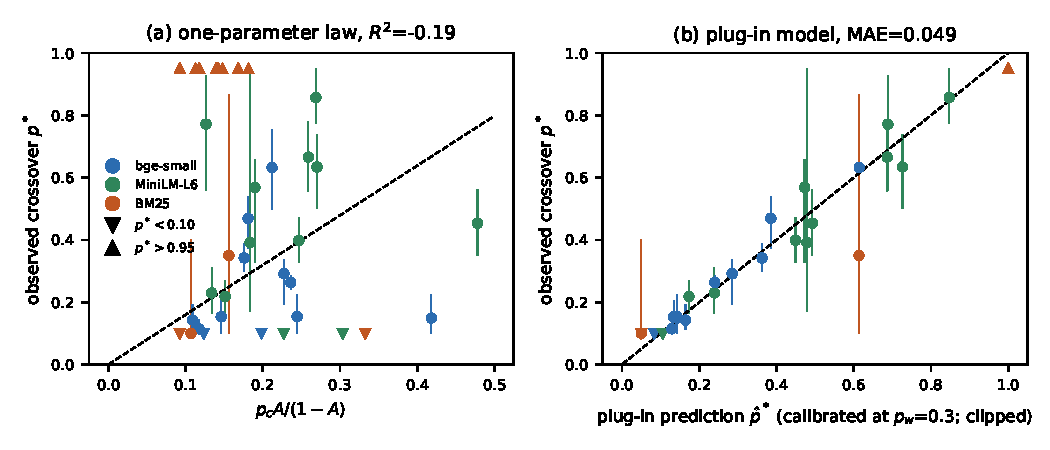
\includegraphics[width=\linewidth]{../figs/crossover_two.pdf}
\caption{Observed crossover against (a) the one-parameter law $p^*=\kappa\,p_cA/(1-A)$ and (b) the plug-in estimate of Eq.~\eqref{eq:pstar} calibrated at $p_w=0.3$. Triangles mark crossovers outside the tested grid; bars are 95\% bootstrap intervals.}
\label{fig:cross}
\end{figure}

\section{Monitoring without labels}
\label{sec:monitor}
In deployment the true error is unknown. The pilot tested one label-free signal and it failed. Here we test five, all computed without ground truth:
(i) the \emph{acceptance rate}, which any deployment observes and which serves as a baseline;
(ii) the \emph{self-written share} of top-1 answers;
(iii) the pilot's signal, the share of answers where a written-back entry wins and the best original post points to a different thread;
(iv) \emph{disagreement with an independent retriever}, the share of asks whose deployed top-1 thread differs from that of a static retriever of a different kind (BM25 for dense deployments, bge for BM25), together with its rise since round 1;
(v) \emph{probe-bank drift}, the share of a fixed bank of 200 asks, queried read-only after each round, whose top-1 thread has changed since the start.

For each forum and retriever, a run (one condition, acceptance rate and order) is labelled harmful if its accuracy over the second half of the stream is below no write-back on the same order. We report the Spearman correlation between each signal (averaged over the second half) and the true accuracy change, pooled over all runs and within a fixed $p_w$, and the AUROC for harmful runs using the signal value at a given round. All values are averaged over the 36 forum--retriever pairs (Table~\ref{tab:monitor}, Figure~\ref{fig:monitor}).

\begin{table}[t]\centering\small
\resizebox{\linewidth}{!}{\begin{tabular}{lrrrrr}\toprule Signal & $\rho$ (all runs) & $\rho$ (fixed $p_w$) & AUROC r2 & AUROC r5 & AUROC r10\\\midrule
Acceptance rate (baseline) & -0.41 & +0.06 & 0.70 & 0.70 & 0.70\\
Self-written share of top-1 & -0.51 & -0.34 & 0.69 & 0.73 & 0.73\\
Pilot signal: self vs.\ human top entry & -0.51 & -0.34 & 0.67 & 0.74 & 0.73\\
Disagreement with independent retriever & -0.32 & -0.21 & 0.54 & 0.58 & 0.60\\
\quad rise since round 1 & -0.13 & -0.07 & 0.54 & 0.57 & 0.58\\
Probe-bank drift & -0.44 & -0.29 & 0.71 & 0.76 & 0.77\\
\bottomrule\end{tabular}}
\caption{Label-free signals against the true change in accuracy. $\rho$: Spearman correlation with the accuracy change (negative means the signal rises as accuracy falls), averaged over forum--retriever pairs. AUROC for identifying harmful runs from the signal after round 2, 5 and 10. Ten rounds.}
\label{tab:monitor}
\end{table}

\begin{figure}[t]\centering
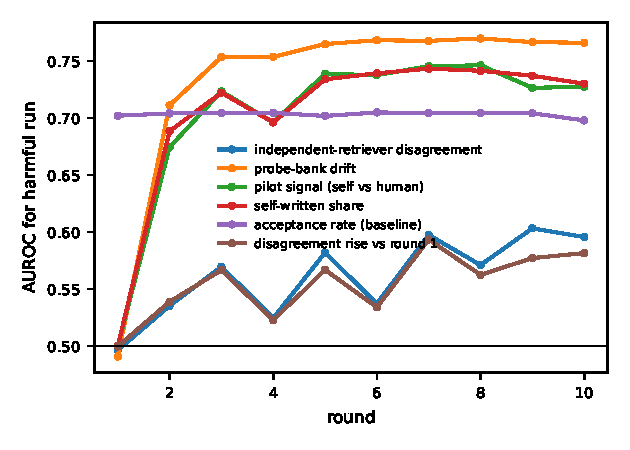
\includegraphics[width=0.55\linewidth]{../figs/monitor_r10_all.pdf}
\caption{AUROC for identifying harmful runs from each label-free signal, by round.}
\label{fig:monitor}
\end{figure}

\paragraph{Results.} The acceptance rate alone gives an AUROC of about 0.70 from the first round, because harm is driven mostly by how often wrong answers are accepted. The self-written share, the pilot signal and probe-bank drift reach 0.72--0.77 after three to five rounds, a small gain over the baseline that arrives late. Within a fixed acceptance rate their correlation with the true accuracy change is weak ($|\rho|\le0.34$). Disagreement with an independent retriever is close to chance (AUROC 0.50--0.61), and its rise since round 1 even more so. The reason is that dense and lexical retrievers already disagree on most asks before any write-back: under bge and BM25 the top-1 thread differs for about 80\% of Android asks. Changes caused by the loop are small against that background. In summary, none of these monitors detects harm in a way that adds much to the acceptance rate. The independent-retriever monitor, which we expected to work best because it does not share the deployed retriever's errors, did not.

\section{Limitations}
\textbf{Simulated acceptance.} User acceptance is the only simulated component, and it is the one that matters most. Real acceptance probably depends on the question, the answer and the user, and acceptance of wrong answers is likely correlated with how plausible they look. Our $p_w$ is a single constant per run. The plug-in model would still apply if the per-entry effects were measured under the real acceptance process, but the crossovers reported here would not.
\textbf{Incomplete ground truth.} CQADupStack duplicate links are incomplete \citep{hoogeveen2015cqadupstack}: an answer we count as wrong may in fact solve the problem. This affects absolute accuracies and could make some ``wrong'' entries harmless, which would raise $p^*$.
\textbf{Short questions.} Asks are post titles, which makes retrieval hard (base top-1 accuracy 9--35\%) and makes written-back entries short. Systems that store longer entries, such as the full question and a generated answer, may behave differently, especially with BM25.
\textbf{Simplified write-back.} Entries point to an existing thread; there is no generation step, so we do not measure errors introduced by an LLM writing the answer. BM25 statistics are not updated as entries are added. The probe bank is drawn from the stream itself.
\textbf{Scope of the model.} The model is first order and is checked on the same simulated data it describes. Calibration at one acceptance rate uses the same orders as the sweep it predicts.

\section{Conclusion}
On real repeat questions from twelve forums, writing accepted answers back into a dense retriever's knowledge base helps only while users reject most wrong answers. The acceptance rate at which it starts to hurt varies from below 0.10 to about 0.86 and is not predicted by base accuracy. It is predicted well by a first-order formula once the per-entry effects of correct and wrong entries are measured, and those effects can be estimated from a small audit. Reopening wrong answers reduces the loss but does not remove it, and the label-free monitors we tried add little to the acceptance rate. For practitioners, the most useful quantities to measure before turning on write-back are the acceptance rate of wrong answers and the per-entry effect of a wrong entry. Monitoring that works without labels remains an open problem.

\section*{Code and data availability}
All data are public (CQADupStack via the BEIR/MTEB distribution on Hugging Face). The code for data preparation, simulation and analysis, the cached per-run results and the scripts that generate every table and figure in this paper will be released on GitHub. Every number in the paper is produced by these scripts from saved runs. The full experiment (embedding twelve forums with two dense models and 9{,}120 simulation runs) runs on a laptop in well under an hour.

\section*{Acknowledgements}
This work uses no employer or customer data. The retrieval setup follows TicketIQ, the author's M.Tech dissertation system.

\bibliography{refs}

\appendix
\section{Full safeguard results}\label{app:safe}
\begin{table}[h]\centering\scriptsize
\begin{tabular}{llrlll}\toprule Forum & Retriever & $p_w$ & Naive & + demotion & + demotion + quarantine\\\midrule
android & bge & 0.3 & +0.54 $\pm$ 0.53 & +1.79 $\pm$ 0.67 & +2.46 $\pm$ 0.90\\
 &  & 0.95 & -1.87 $\pm$ 0.65 & -0.43 $\pm$ 0.67 & -0.44 $\pm$ 0.72\\
 & MiniLM & 0.3 & +0.54 $\pm$ 0.28 & +0.92 $\pm$ 0.20 & +0.84 $\pm$ 0.36\\
 &  & 0.95 & -0.29 $\pm$ 0.24 & +0.31 $\pm$ 0.23 & +0.30 $\pm$ 0.26\\
\addlinespace[1pt]
english & bge & 0.3 & +1.25 $\pm$ 0.45 & +1.95 $\pm$ 0.38 & +2.16 $\pm$ 0.49\\
 &  & 0.95 & -0.81 $\pm$ 0.44 & +0.64 $\pm$ 0.36 & +0.61 $\pm$ 0.37\\
 & MiniLM & 0.3 & +1.84 $\pm$ 0.46 & +2.83 $\pm$ 0.26 & +2.85 $\pm$ 0.47\\
 &  & 0.95 & -0.21 $\pm$ 0.42 & +1.44 $\pm$ 0.28 & +1.34 $\pm$ 0.26\\
\addlinespace[1pt]
gaming & bge & 0.3 & -0.44 $\pm$ 0.31 & -0.05 $\pm$ 0.26 & +0.35 $\pm$ 0.28\\
 &  & 0.95 & -1.92 $\pm$ 0.20 & -0.92 $\pm$ 0.22 & -0.93 $\pm$ 0.23\\
 & MiniLM & 0.3 & +0.15 $\pm$ 0.10 & +0.39 $\pm$ 0.12 & +0.67 $\pm$ 0.19\\
 &  & 0.95 & -0.45 $\pm$ 0.23 & +0.03 $\pm$ 0.20 & +0.03 $\pm$ 0.21\\
\addlinespace[1pt]
gis & bge & 0.3 & -0.53 $\pm$ 0.32 & +0.06 $\pm$ 0.27 & +0.02 $\pm$ 0.27\\
 &  & 0.95 & -2.23 $\pm$ 0.33 & -1.08 $\pm$ 0.24 & -1.11 $\pm$ 0.27\\
 & MiniLM & 0.3 & -0.18 $\pm$ 0.18 & -0.07 $\pm$ 0.13 & -0.08 $\pm$ 0.13\\
 &  & 0.95 & -0.55 $\pm$ 0.18 & -0.30 $\pm$ 0.15 & -0.30 $\pm$ 0.15\\
\addlinespace[1pt]
mathematica & bge & 0.3 & -0.87 $\pm$ 0.24 & -0.30 $\pm$ 0.30 & -0.23 $\pm$ 0.30\\
 &  & 0.95 & -2.58 $\pm$ 0.30 & -1.41 $\pm$ 0.31 & -1.41 $\pm$ 0.31\\
 & MiniLM & 0.3 & -0.19 $\pm$ 0.29 & +0.40 $\pm$ 0.26 & +0.29 $\pm$ 0.29\\
 &  & 0.95 & -1.15 $\pm$ 0.27 & -0.42 $\pm$ 0.22 & -0.43 $\pm$ 0.21\\
\addlinespace[1pt]
physics & bge & 0.3 & -0.03 $\pm$ 0.28 & +0.56 $\pm$ 0.34 & +0.59 $\pm$ 0.32\\
 &  & 0.95 & -1.70 $\pm$ 0.39 & -0.72 $\pm$ 0.32 & -0.73 $\pm$ 0.32\\
 & MiniLM & 0.3 & +0.32 $\pm$ 0.27 & +0.64 $\pm$ 0.21 & +0.72 $\pm$ 0.16\\
 &  & 0.95 & -0.74 $\pm$ 0.29 & +0.04 $\pm$ 0.32 & +0.03 $\pm$ 0.32\\
\addlinespace[1pt]
programmers & bge & 0.3 & +0.27 $\pm$ 0.29 & +0.88 $\pm$ 0.25 & +1.00 $\pm$ 0.15\\
 &  & 0.95 & -1.73 $\pm$ 0.28 & -0.42 $\pm$ 0.27 & -0.41 $\pm$ 0.27\\
 & MiniLM & 0.3 & +0.31 $\pm$ 0.31 & +0.60 $\pm$ 0.27 & +0.51 $\pm$ 0.28\\
 &  & 0.95 & -0.48 $\pm$ 0.24 & +0.07 $\pm$ 0.31 & +0.07 $\pm$ 0.31\\
\addlinespace[1pt]
stats & bge & 0.3 & -0.82 $\pm$ 0.24 & -0.35 $\pm$ 0.15 & -0.19 $\pm$ 0.17\\
 &  & 0.95 & -1.73 $\pm$ 0.22 & -1.18 $\pm$ 0.24 & -1.18 $\pm$ 0.24\\
 & MiniLM & 0.3 & -0.33 $\pm$ 0.26 & -0.19 $\pm$ 0.24 & -0.22 $\pm$ 0.21\\
 &  & 0.95 & -1.11 $\pm$ 0.21 & -0.56 $\pm$ 0.30 & -0.57 $\pm$ 0.29\\
\addlinespace[1pt]
tex & bge & 0.3 & -0.81 $\pm$ 0.17 & -0.25 $\pm$ 0.24 & +0.13 $\pm$ 0.38\\
 &  & 0.95 & -2.62 $\pm$ 0.18 & -1.49 $\pm$ 0.23 & -1.49 $\pm$ 0.24\\
 & MiniLM & 0.3 & -0.21 $\pm$ 0.15 & +0.13 $\pm$ 0.15 & +0.36 $\pm$ 0.17\\
 &  & 0.95 & -1.03 $\pm$ 0.11 & -0.42 $\pm$ 0.16 & -0.41 $\pm$ 0.16\\
\addlinespace[1pt]
unix & bge & 0.3 & -0.32 $\pm$ 0.25 & +0.58 $\pm$ 0.39 & +0.73 $\pm$ 0.36\\
 &  & 0.95 & -2.68 $\pm$ 0.57 & -1.03 $\pm$ 0.51 & -1.03 $\pm$ 0.51\\
 & MiniLM & 0.3 & +0.62 $\pm$ 0.24 & +0.73 $\pm$ 0.23 & +0.82 $\pm$ 0.24\\
 &  & 0.95 & -0.47 $\pm$ 0.24 & +0.27 $\pm$ 0.19 & +0.21 $\pm$ 0.20\\
\addlinespace[1pt]
webmasters & bge & 0.3 & -0.45 $\pm$ 0.35 & +0.04 $\pm$ 0.33 & +0.23 $\pm$ 0.35\\
 &  & 0.95 & -1.79 $\pm$ 0.28 & -0.93 $\pm$ 0.41 & -0.92 $\pm$ 0.41\\
 & MiniLM & 0.3 & +0.51 $\pm$ 0.35 & +0.85 $\pm$ 0.35 & +1.20 $\pm$ 0.44\\
 &  & 0.95 & -0.32 $\pm$ 0.26 & +0.23 $\pm$ 0.36 & +0.24 $\pm$ 0.35\\
\addlinespace[1pt]
wordpress & bge & 0.3 & -0.27 $\pm$ 0.16 & +0.01 $\pm$ 0.11 & +0.17 $\pm$ 0.14\\
 &  & 0.95 & -0.99 $\pm$ 0.34 & -0.43 $\pm$ 0.41 & -0.43 $\pm$ 0.41\\
 & MiniLM & 0.3 & +0.15 $\pm$ 0.28 & +0.19 $\pm$ 0.18 & +0.15 $\pm$ 0.17\\
 &  & 0.95 & -0.11 $\pm$ 0.24 & +0.11 $\pm$ 0.23 & +0.11 $\pm$ 0.23\\
\bottomrule\end{tabular}
\caption{Paired change in top-1 accuracy (points, 95\% interval over ten orders) relative to no write-back, for the dense retrievers.}
\label{tab:safe}
\end{table}
\end{document}
